\documentclass[aspectratio=169]{beamer}
\usepackage[utf8]{inputenc}
\usepackage{hyperref}
\usepackage{amsmath,amsfonts,amsthm,bm}
\usepackage{color}
\usepackage{graphicx} % Allows including images
\usepackage{subcaption}
\usepackage{booktabs} % Allows the use of \toprule, \midrule and \bottomrule in tables
\usepackage{tikz}
\usetikzlibrary{automata,positioning,shapes.geometric, arrows}
%\usepackage{pgfplots}
\usepackage{adjustbox}
\usepackage{listings}
\usepackage{courier}
\usepackage[version=4]{mhchem}
\usepackage{array}
\usepackage{physics}

\lstset{ %
  basicstyle=\scriptsize\ttfamily, % fonts that are used for the code
  breakatwhitespace=false,         % sets if automatic breaks should only happen at whitespace
  %breaklines=true,                 % sets automatic line breaking
  %captionpos=b,                    % sets the caption-position to bottom
  commentstyle=\color{gray}\textit,    % comment style
  keepspaces=true,                 % keeps spaces in text, useful for keeping indentation of code (possibly needs columns=flexible)
  keywordstyle=\color{blue},       % keyword style
  language=Python,                 % the language of the code
  %otherkeywords={*,...},          % if you want to add more keywords to the set
  rulecolor=\color{black},         % if not set, the frame-color may be changed on line-breaks within not-black text (e.g. comments (green here))
  showspaces=false,                % show spaces everywhere adding particular underscores; it overrides 'showstringspaces'
  showstringspaces=false,          % underline spaces within strings only
  showtabs=false,                  % show tabs within strings adding particular underscores
  stringstyle=\color{red}, % string literal style
  tabsize=4,	                   % sets default tabsize to 2 spaces
  columns=fixed                    % Using fixed column width (for e.g. nice alignment)
}

\hypersetup{
    colorlinks=true,
    linkcolor=red,
    filecolor=magenta,      
    urlcolor=red,
}

\DeclareMathOperator*{\argmax}{argmax}
\DeclareMathOperator*{\argmin}{argmin}
\let \vec \mathbf

\newcommand{\classname}{NANO266}
\newcommand{\classyear}{Fall 2024}
\mode<presentation> {
    \usetheme{CambridgeUS}
    \setbeamertemplate{footline}[text line]{%
      \parbox{\linewidth}{\vspace*{-8pt}\classname\hfill\classyear\hfill\insertpagenumber}}

    %\setbeamertemplate{footline}[page number]
    \setbeamertemplate{navigation symbols}{}
}


\title[\classname Exchange-Correlation Functionals]{\classname~- Quantum Mechanical Modeling of Materials and Nanostructures\\Exchange-Correlation Functionals}

\author{Shyue Ping Ong}
\institute[UCSD]{University of California, San Diego\\
\medskip
}
\date{\classyear} % Date, can be changed to a custom date

\begin{document}


\begin{frame}
    \titlepage % Print the title page as the first slide
\end{frame}


\begin{frame}{Beyond LDA}

LDA uses local density $\rho$ from homogenous electron gas.\newline
\newline
Next step: Let’s add a gradient of the density!\newline
\newline
Generalized gradient approximation (GGA)
\begin{equation*}
    E_{xc}^{GGA}[\rho^\uparrow, \rho^\downarrow] = \int d \vec{r} \rho(\vec{r})\varepsilon_{xc}(\rho^\uparrow, \rho^\downarrow, |\nabla\rho^\uparrow|, |\nabla\rho^\downarrow|)
\end{equation*}

\end{frame}

\begin{frame}{There is more than one GGA}
\begin{itemize}
    \item BLYP, 1988: Exchange by Axel Becke based on energy density of atoms, one parameter + Correlation by Lee-Yang-Parr.\cite{beckeDensityfunctionalExchangeenergyApproximation1988}
    \item PW91, 1991: Perdew-Wang 91 Parametrization of real-space cut-off procedure.\cite{burkeDerivationGeneralizedGradient1998}
    \item PBE, 1996: Perdew-Burke-Ernzerhof (re-parametrization and simplification of PW91)\cite{perdewGeneralizedGradientApproximation1996}
    \item RPBE, 1999: revised PBE, improves surface energetics
    \item PBEsol, 2008: Revised PBE for solids.\cite{perdewRestoringDensityGradientExpansion2008a}

\end{itemize}


\end{frame} 

\begin{frame}{Performance of GGA}
\begin{columns}
\column{0.65\textwidth}
GGA tends to correct LDA overbinding $\rightarrow$
Better bond lengths, lattice parameters, atomization energies, etc.

\column{0.35\textwidth}
\begin{figure}
    \centering
    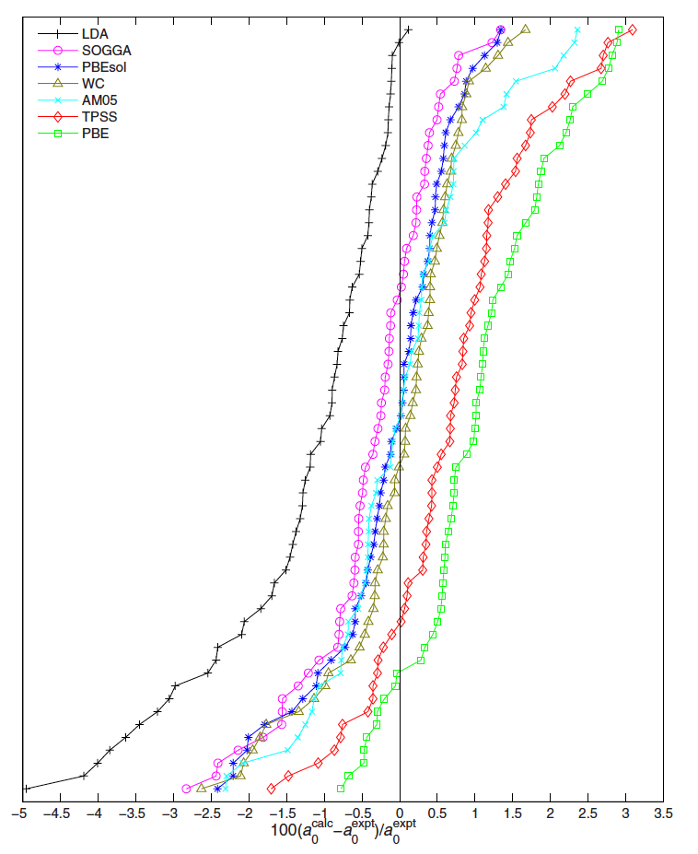
\includegraphics[width=\linewidth]{lectures/figures/5_bond_lengths.png}
\end{figure}

\end{columns}
\end{frame} 

\begin{frame}{Meta-GGAs}
Meta-GGAs (including the kinetic energy density corrections)
\begin{equation*}
    E_{xc}^{GGA}[\rho^\uparrow, \rho^\downarrow] = \int d \vec{r} \rho(\vec{r})\varepsilon_{xc}(\rho^\uparrow, \rho^\downarrow, |\nabla\rho^\uparrow|, |\nabla\rho^\downarrow|, \nabla^2\rho^\uparrow, \nabla^2\rho^\downarrow)
\end{equation*}

Example: TPSS,\cite{taoClimbingDensityFunctional2003} SCAN,\cite{sunStronglyConstrainedAppropriately2015} etc.

\end{frame} 


\begin{frame}{State-of-the-art: Strongly Constrained and Appropriately Normed (SCAN) functional}

\begin{columns}
\column{0.8\textwidth}
Recovers 17 exact constraints expected for a semi-local DFT functional (e.g., slowly varying gas limit).\cite{sunStronglyConstrainedAppropriately2015}

Significantly improved geometries and energetics.\cite{sunAccurateFirstprinciplesStructures2016}
\begin{figure}
    \centering
    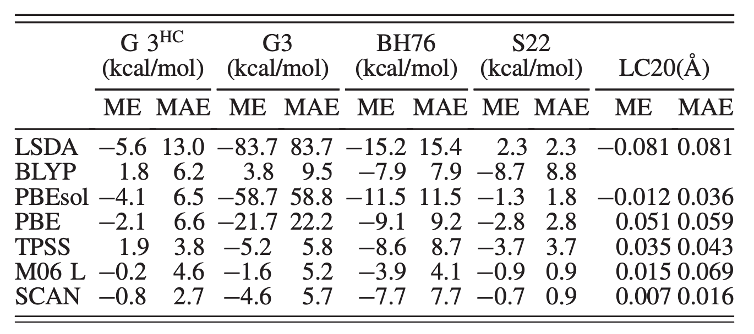
\includegraphics[width=0.8\linewidth]{lectures/figures/6_scan_performance.png}
\end{figure}
 
\column{0.2\textwidth}
\begin{figure}
    \centering
    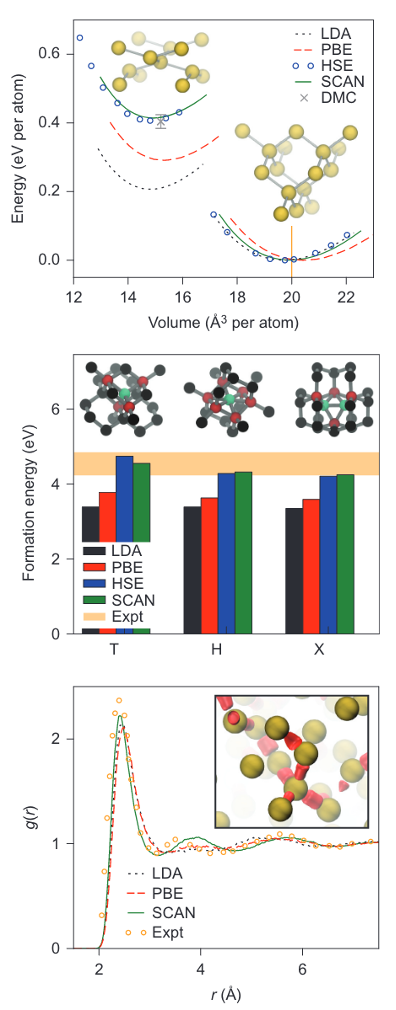
\includegraphics[width=0.8\linewidth]{lectures/figures/6_scan_performance_2.png}
\end{figure}
\end{columns} 

\end{frame}

\begin{frame}{Orbital-dependent methods}
DFT+$U$\cite{anisimovBandTheoryMott1991,anisimovDensityFunctionalTheoryNio1993,dudarevElectronenergylossSpectraStructural1998}
\begin{itemize}
    \item Treat strong on-site Coulomb interaction of localized electrons, e.g., $d$ and $f$ electrons (incorrectly described by LDA or GGA) with an additional Hubbard-like term. 
    \item Strength of on-site interactions usually described by $U$ (on site Coulomb) and $J$ (on site exchange), which can be self-consistently extracted from ab initio calculations,\cite{cococcioniLinearResponseApproach2005} but usually are obtained semi-empirically, e.g., fitting to experimental formation energies or band gaps.
\end{itemize}
\begin{equation*}
    E_{DFT+U} = E_{DFT} + \sum_\sigma \frac{U_{eff}}{2} \left[ \left( \sum_{m_1} \rho_{m_1,m_1}^\sigma \right) - \left( \sum_{m_1,m_2} \rho_{m_1,m_2}^\sigma\rho_{m_2,m_1}^\sigma \right)  \right]
\end{equation*}

\end{frame} 

\begin{frame}{Obtaining $U$ values}
\begin{columns}
\column{0.6\textwidth}
Option 1: Fit it yourself, either using linear response approach or to some experimental data that you have for your problem at hand.\newline
\newline
Option 2: Use well-tested values in the literature, e.g., from \href{https://docs.materialsproject.org/methodology/materials-methodology/calculation-details/gga+u-calculations/hubbard-u-values}{Materials Project} (though you should use caution!)
\column{0.4\textwidth}

\begin{figure}
    \centering
    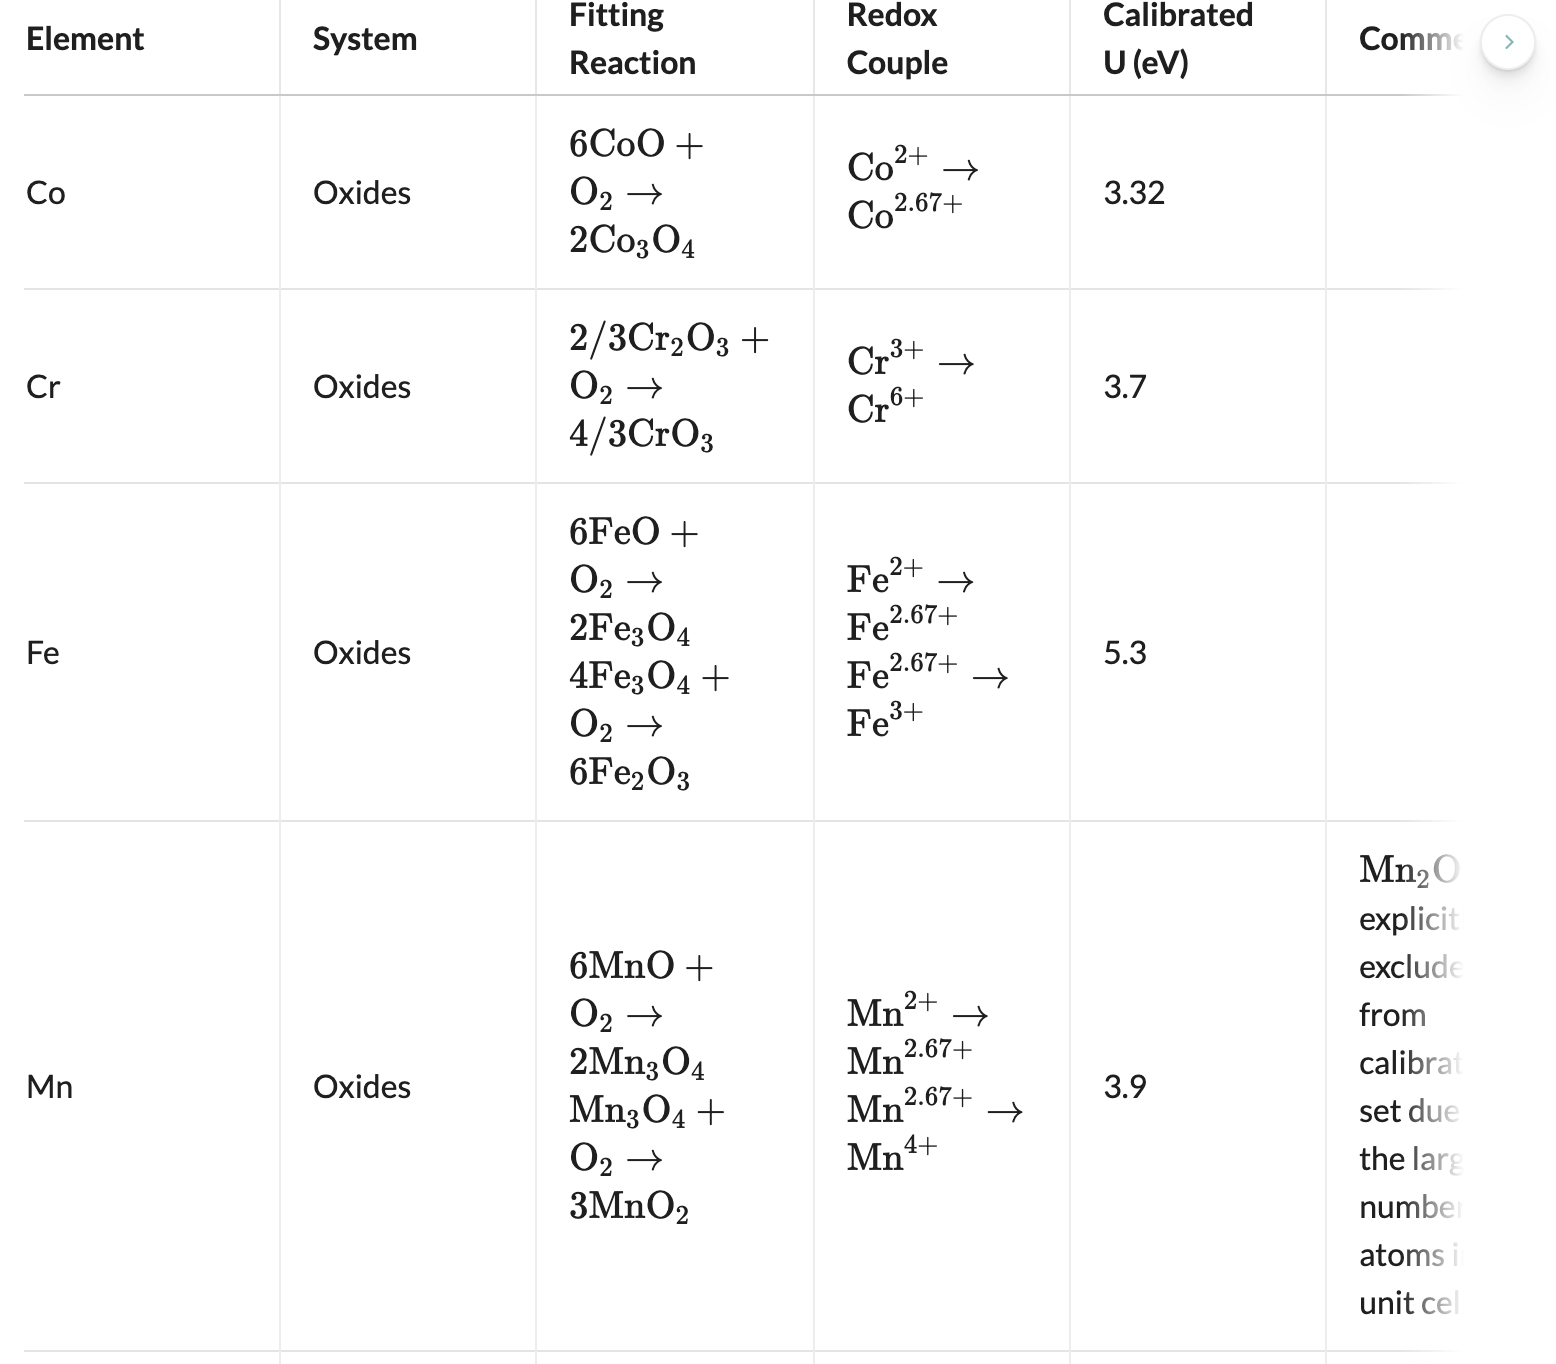
\includegraphics[width=0.9\linewidth]{lectures/figures/6_mp_u_values.png}
    \caption{Fitted by a UCSD NanoEngineering Professor for the Materials Project.}
\end{figure}
\end{columns} 

\end{frame} 


\begin{frame}{Hybrids}
\begin{figure}
    \centering
    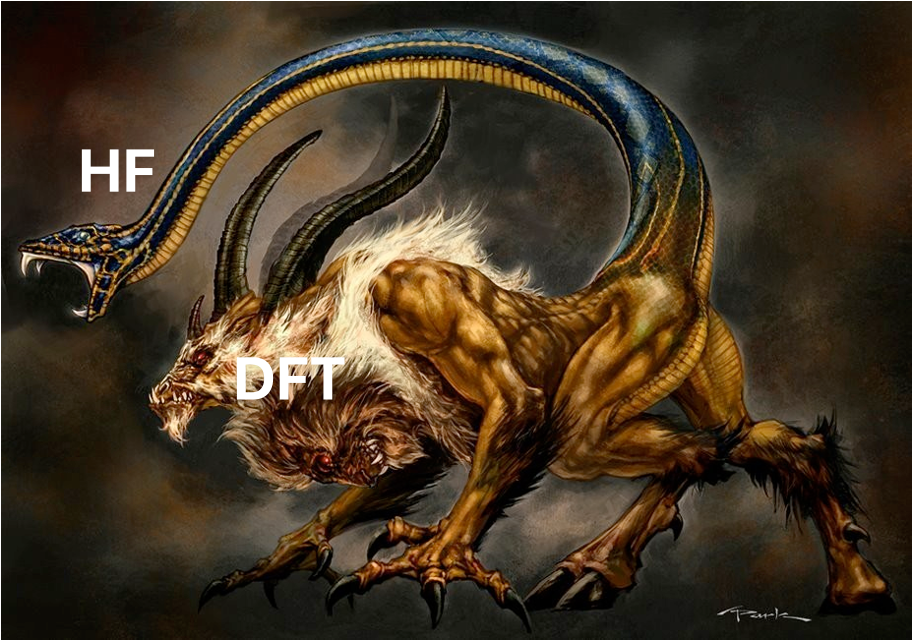
\includegraphics[width=0.5\linewidth]{lectures/figures/6_chimera.png}
    \caption{Chimera from God of War (memories of times when I was still a carefree graduate student)}
\end{figure}
\end{frame} 


\begin{frame}{Rationale for Hybrids}
Semi-local DFT suffer from the dreaded self-interaction error (SIC), spurious interaction of the electron not completely cancelled with approximate $E_{xc}$.
\begin{eqnarray*}
    E^{DFT}_{ee} & = & \frac{1}{2} \int \int \frac{\rho(\vec{r'})\rho(\vec{r})}{|\vec{r}-\vec{r'}|} d\vec{r}d\vec{r'}
\end{eqnarray*}

In contrast, HF exchange cancels self-interaction by construction.

\begin{eqnarray*}
    E^{HF}_{x} & = & - \frac{1}{2} \int \int \frac{\rho(\vec{r'})\rho(\vec{r})}{|\vec{r}-\vec{r'}|} d\vec{r}d\vec{r'}
\end{eqnarray*}
\end{frame} 

\begin{frame}{Flavors of Hybrid Functionals}
\begin{columns}
\column{0.5\textwidth}
B3LYP (Becke 3-parameter, Lee-Yang-Parr)\cite{beckeDensityFunctionalThermochemistry1993}
\begin{eqnarray*}
    E^{B3LYP}_{xc} & = & E_x^{LDA} + a_0 (E_x^{HF} - E_x^{LDA})\\
    & + & a_x (E_x^{GGA}-E_x^{LDA}) \\
    & +&  E_c^{LDA} +(E_c^{GGA} - E_c^{LDA})
\end{eqnarray*}
where $a_0 = -0.2$, $a_x = 0.72$ and $a_c = 0.81$.
\begin{itemize}
    \item Arguably the most popular functional in quantum chemistry (the 8th most cited paper in all fields).
    \item Originally fitted from a set of atomization energies, ionization potentials, proton affinities and total atomic energies.
\end{itemize}
\column{0.5\textwidth}

PBE0:
\begin{eqnarray*}
    E^{PBE0}_{xc} = 0.25E_x^{HF} + 0.75 E_x^{PBE} + E_c^{PBE}
\end{eqnarray*}
HSE (Heyd-Scuseria-Ernzerhof) (2006):\cite{heydHybridFunctionalsBased2003,heydErratumHybridFunctionals2006}
\begin{eqnarray*}
    E^{HSE}_{xc} & = & a E_x^{HF,SR}(\omega) +  (1-a) E_x^{PBE,SR}(\omega) \\
    &+& E_x^{PBE,LR}(\omega) + E_c^{PBE}
\end{eqnarray*}

Effectively PBE0, but with an adjustable parameter $\omega$ ($\sim 0.2$) controlling the range of the exchange interaction, aka a \textit{screened} hybrid functional. Works remarkably well for extended systems like solids.
\end{columns} 


\end{frame} 

\begin{frame}{Do hybrids work?}
\begin{figure}
    \centering
    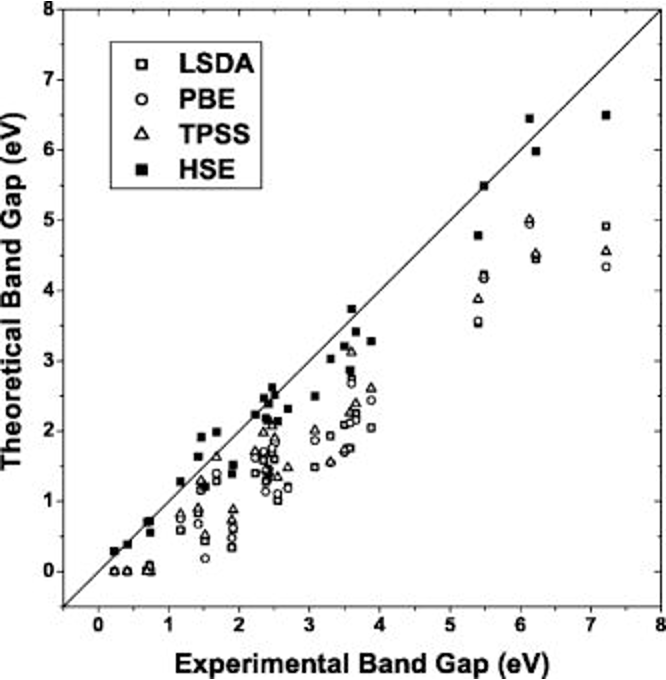
\includegraphics[width=0.4\linewidth]{lectures/figures/6_HSE_bandgaps.png}
        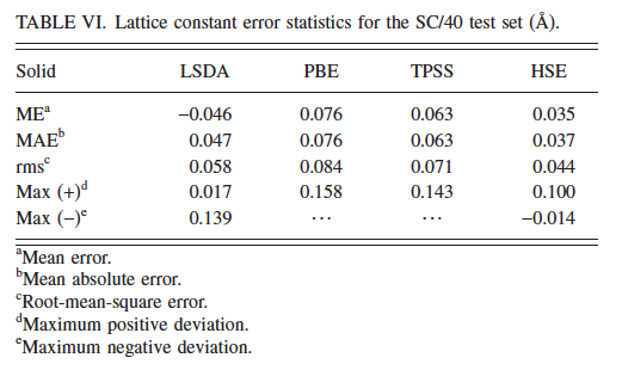
\includegraphics[width=0.55\linewidth]{lectures/figures/6_HSE_bandgap_MAE.png}
    \caption{Ref \cite{heydEnergyBandGaps2005}.}
    \label{fig:enter-label}
\end{figure}
\end{frame} 

\begin{frame}{Do hybrids work?}
\begin{figure}
    \centering
    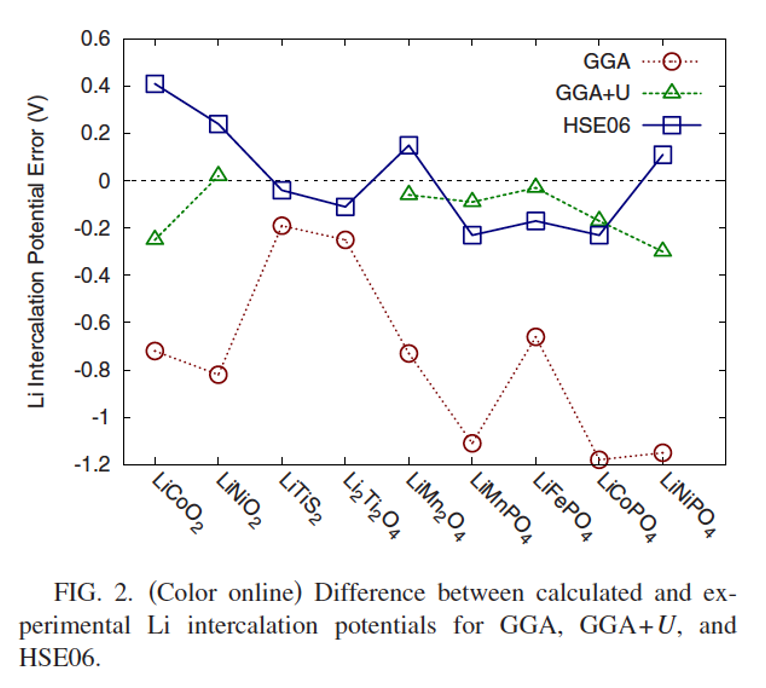
\includegraphics[width=0.45\linewidth]{lectures/figures/6_hse_voltage.png}
        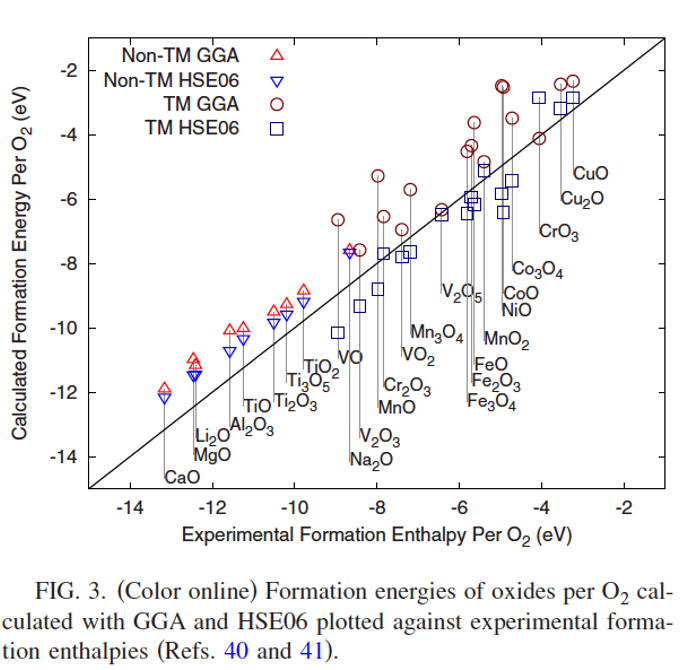
\includegraphics[width=0.4\linewidth]{lectures/figures/6_hse_oxidation_energies.png}
    \caption{Ref \cite{chevrierHybridDensityFunctional2010}.}
    \label{fig:enter-label}
\end{figure}
\end{frame} 

\begin{frame}{How to choose a XC functional}
\begin{figure}
    \centering
    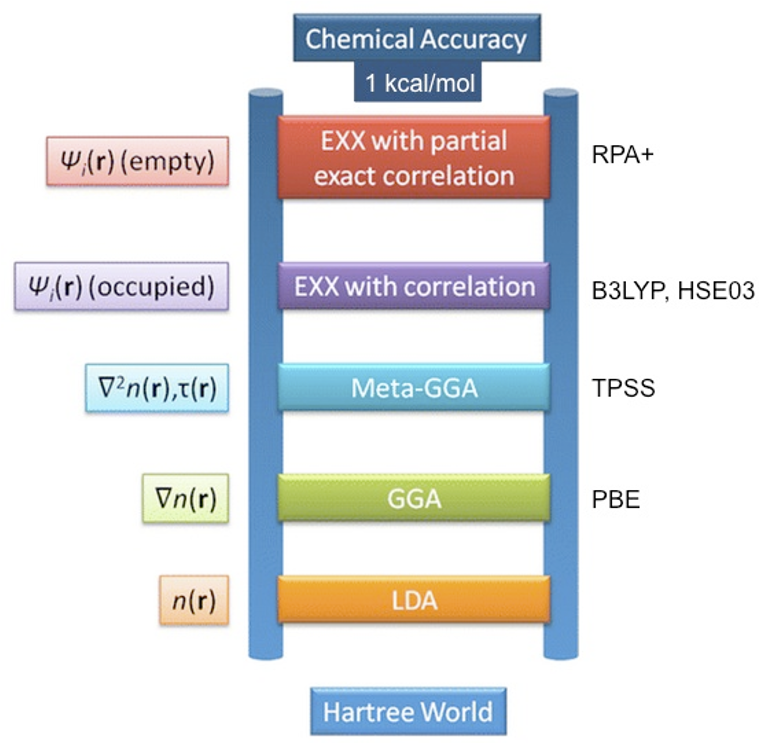
\includegraphics[width=0.4\linewidth]{lectures/figures/6_jacobs_ladder.png}
    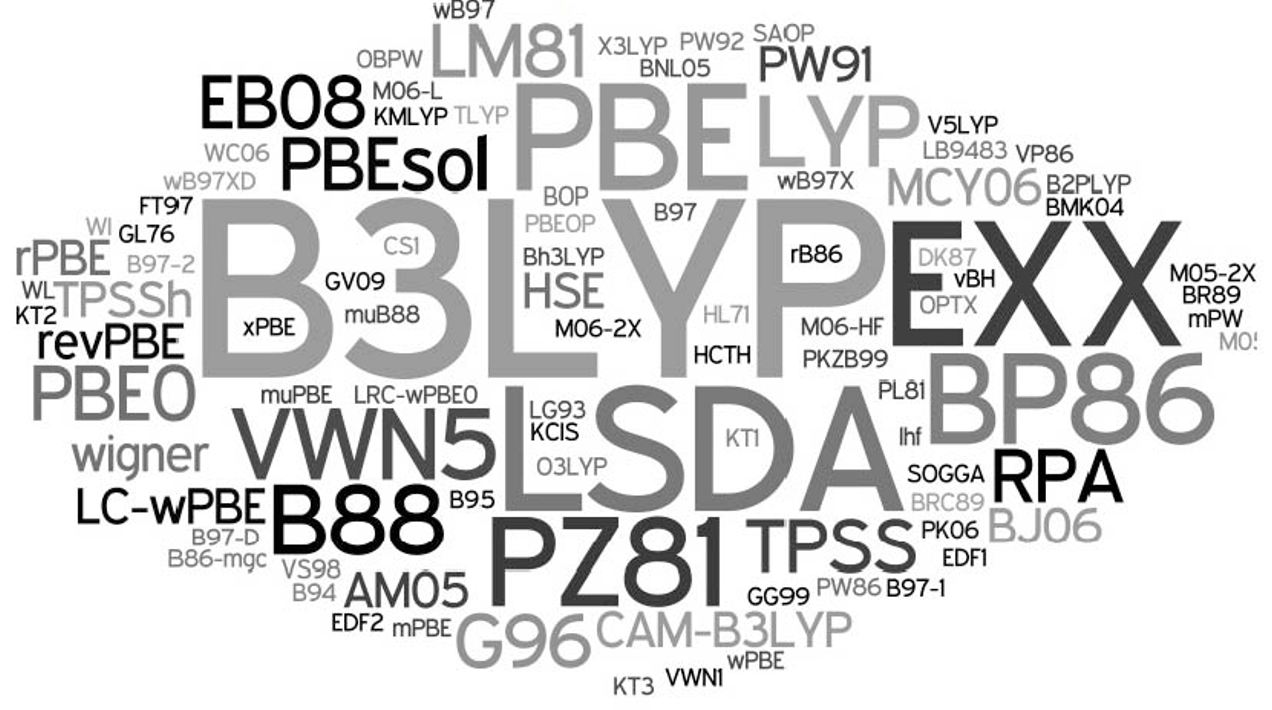
\includegraphics[width=0.58\linewidth]{lectures/figures/6_functional_choices.png}
\end{figure}
\end{frame} 

\begin{frame}{Recap: Tradeoff Trinity}
\begin{figure}
    \centering
    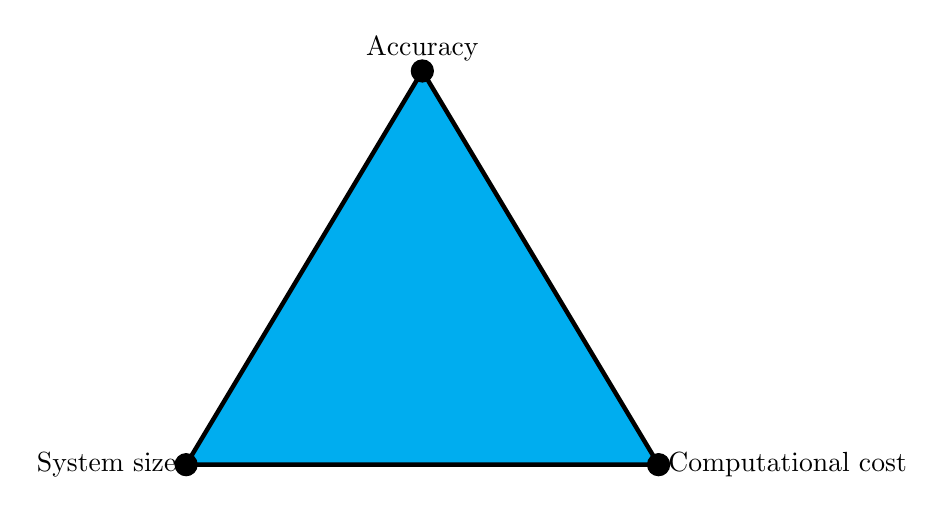
\begin{tikzpicture}
    \filldraw[color=black, fill=cyan, ultra thick] (4,0) -- (10,0) -- (7,5) -- cycle;
    \filldraw[black] (4,0) circle (4pt) node[anchor=east]{System size};
    \filldraw[black] (10,0) circle (4pt) node[anchor=west]{Computational cost};
    \filldraw[black] (7,5) circle (4pt) node[anchor=south]{Accuracy};
    \end{tikzpicture}
    \caption{Choose two (sometimes you only get one)}
\end{figure}

\end{frame}

\begin{frame}{Functional Comparisons: Structural Parameters}
\begin{columns}
\column{0.6\textwidth}
\begin{figure}
    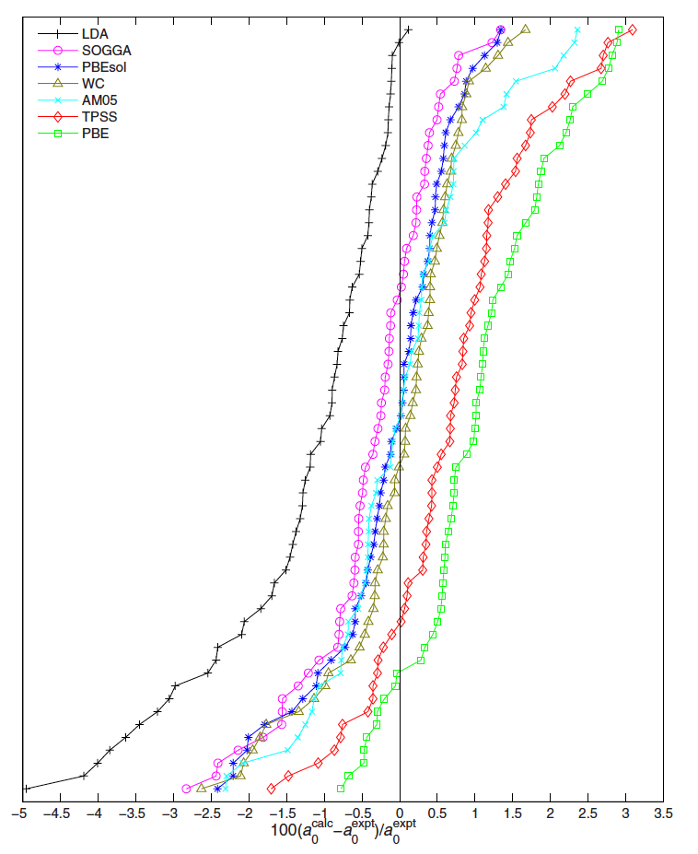
\includegraphics[width=0.55\linewidth]{lectures/figures/5_bond_lengths.png}
    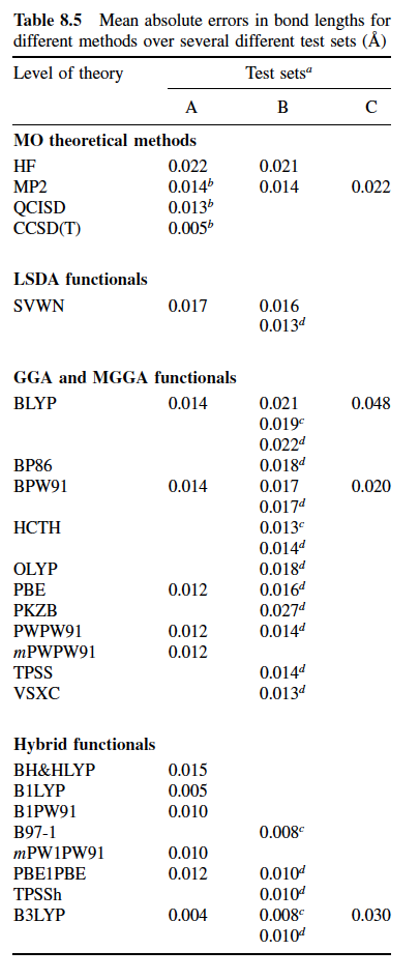
\includegraphics[width=0.3\linewidth]{lectures/figures/6_bond_lengths.png}
    \caption{Ref \cite{haasCalculationLatticeConstant2009, cramerEssentialsComputationalChemistry2004}.}
\end{figure}
\column{0.4\textwidth}
\begin{figure}
    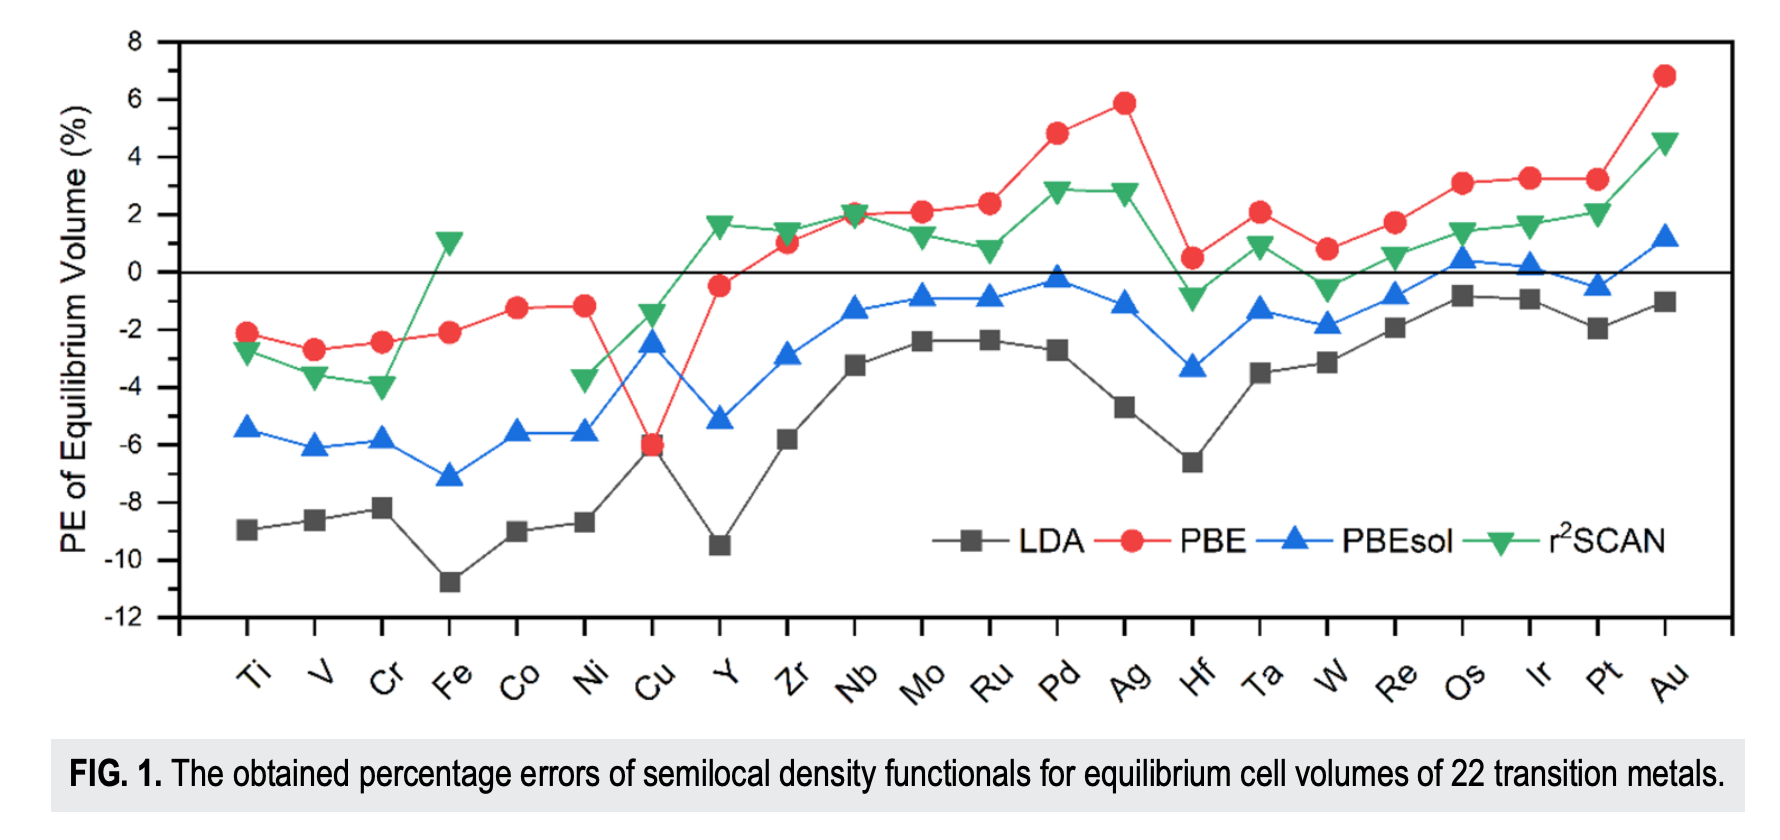
\includegraphics[width=0.9\linewidth]{lectures/figures/6_equilibrium_vol.png}
    \caption{Ref \cite{liuAssessingR2SCANMetaGGA2024}.}
\end{figure}
\begin{itemize}
    \item LDA overbinds.
    \item GGA tends to underbind.
    \item Modified GGAs and meta-GGAs do much better.
\end{itemize}
\end{columns} 
\end{frame} 


\begin{frame}{Functional Comparisons: Cohesive Energies}
\begin{columns}
\column{0.3\textwidth}
\begin{figure}
    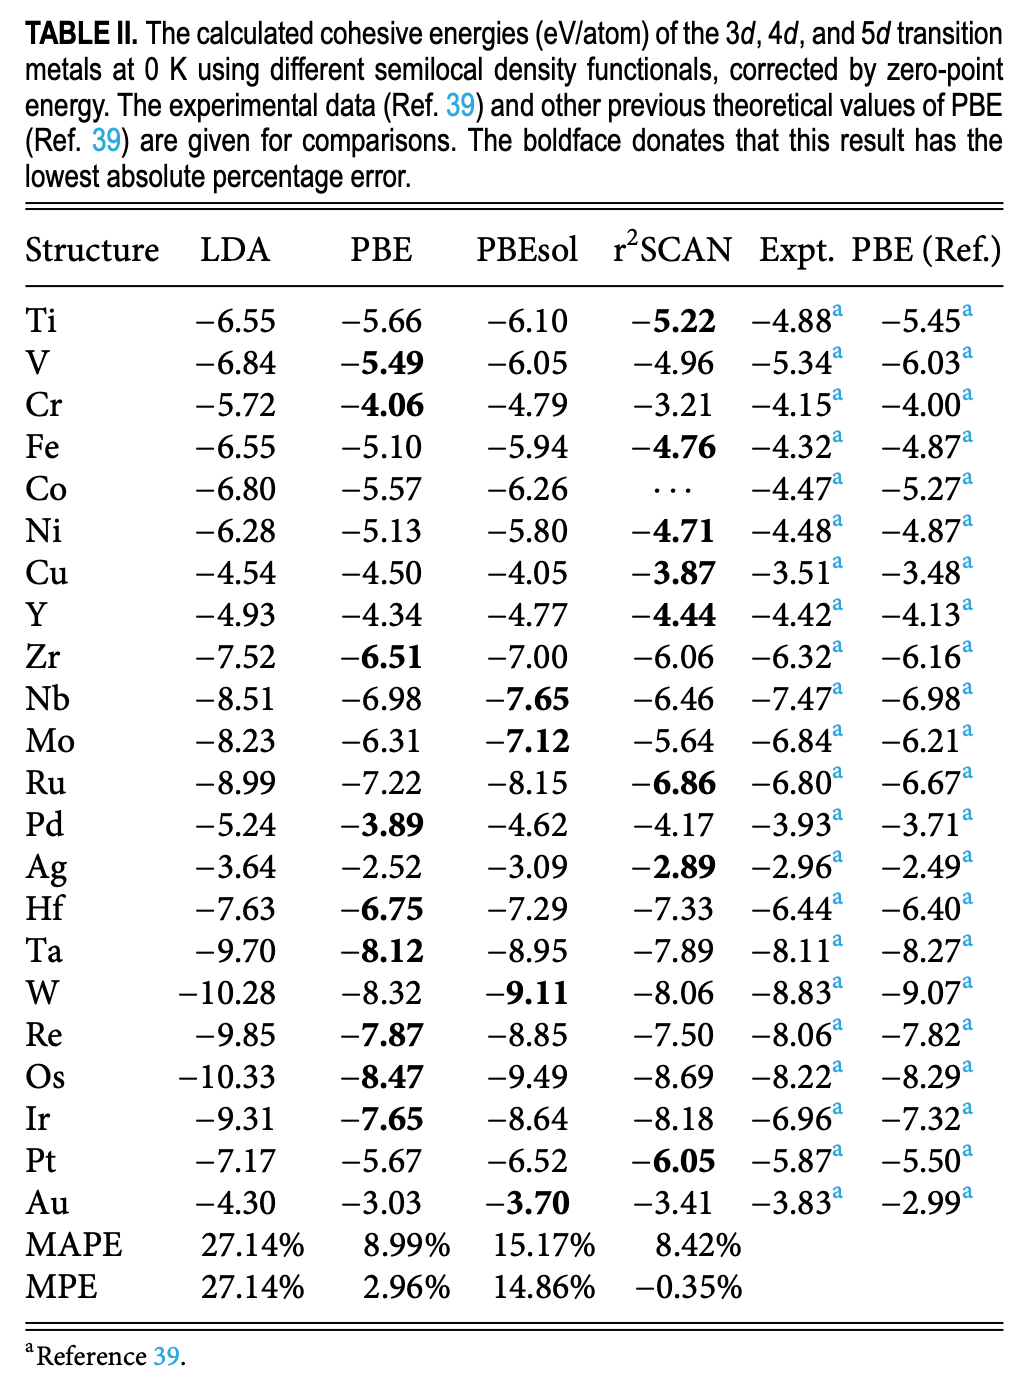
\includegraphics[width=\linewidth]{lectures/figures/6_cohesive_energies.png}
\end{figure}
\column{0.7\textwidth}
\begin{itemize}
    \item Ref \cite{liuAssessingR2SCANMetaGGA2024}.
    \item LDA cohesive energies way too low, i.e., overbinding.
    \item PBE does better but still overbinds on average.
    \item r2SCAN performs much better.
\end{itemize}
\end{columns} 
\end{frame} 


\begin{frame}{Functional Comparisons: Ground State Predictions}
\begin{columns}
\column{0.65\textwidth}
\begin{figure}
    \centering
    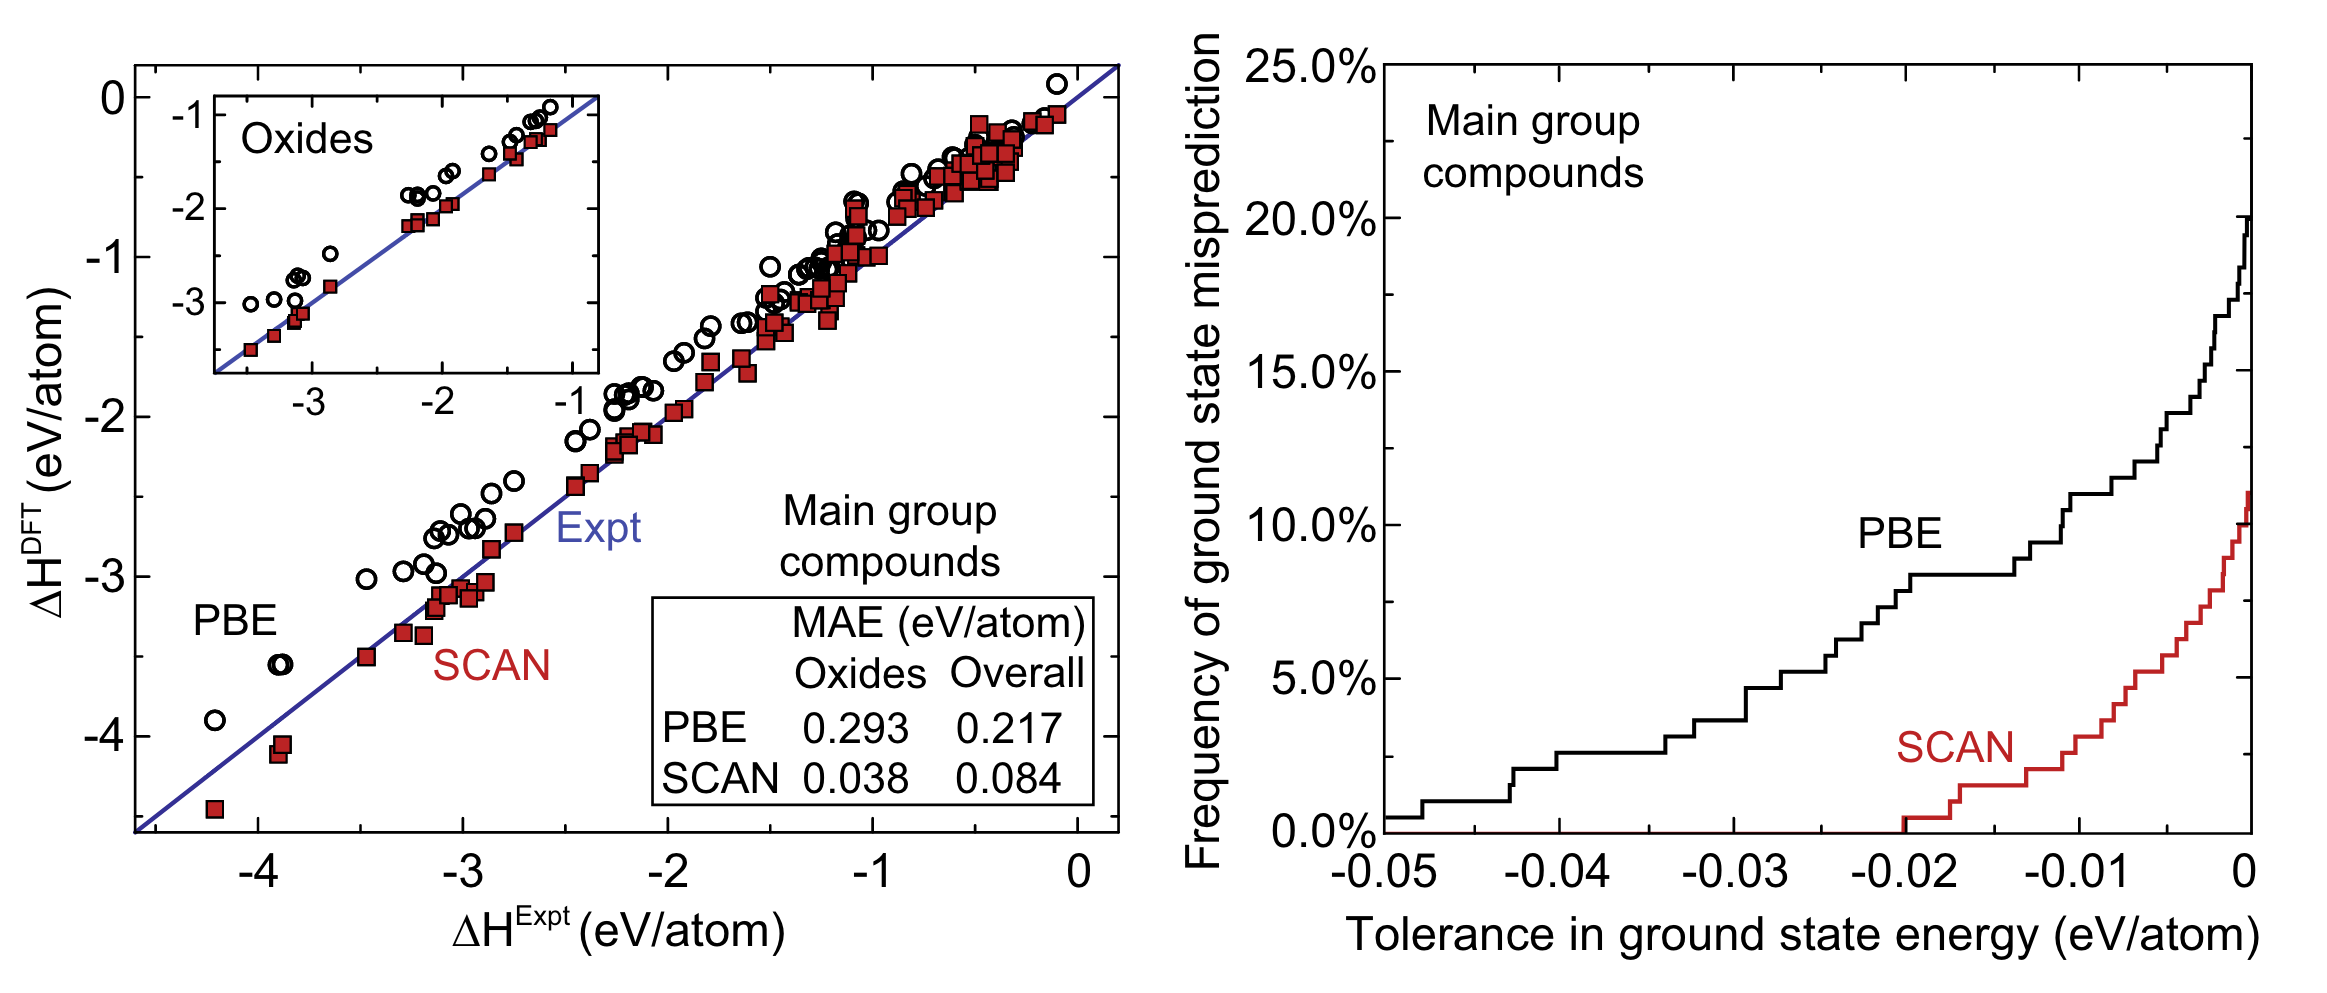
\includegraphics[width=\linewidth]{lectures/figures/6_ground_states.png}
    \caption{Ref \cite{zhangEfficientFirstprinciplesPrediction2017}.}
\end{figure}
\column{0.35\textwidth}
\begin{itemize}
    \item Atomic energy: -1894.074 Ry
    \item Fcc V : -1894.7325 Ry
    \item Bcc V : -1894.7125 Ry
    \item Cohesive energy = 0.638 Ry (0.03\% of total E)
    \item Fcc/bcc difference = 0.02 Ry (0.001\% of total E)
    \item Mixing energies $\sim 10^{-6}$ of total E
\end{itemize}
\end{columns} 

\end{frame} 


\begin{frame}{Functional Comparisons: Atomization energies, ionization energies and electron affinities of molecules}
\begin{figure}
    \centering
    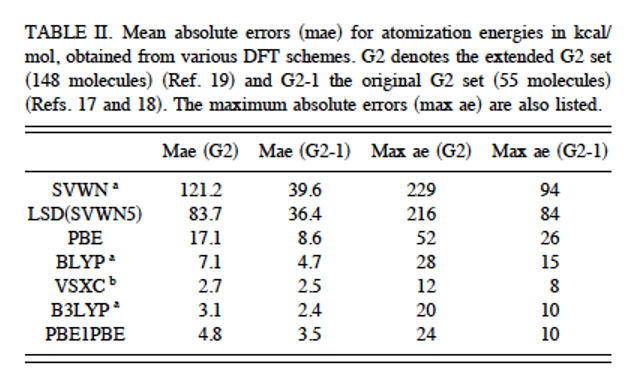
\includegraphics[width=0.3\linewidth]{lectures/figures/6_atomization_energies.png}
    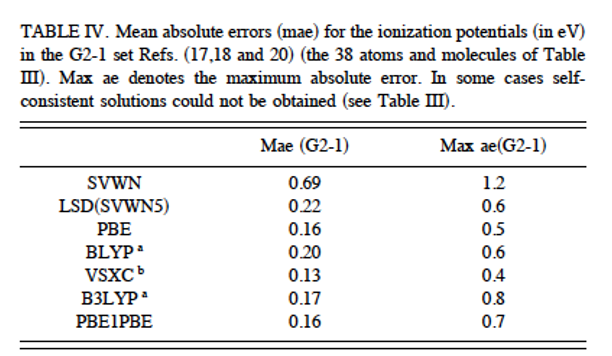
\includegraphics[width=0.3\linewidth]{lectures/figures/6_IEs.png}
    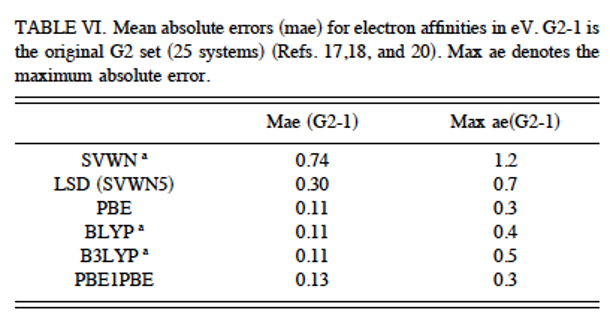
\includegraphics[width=0.3\linewidth]{lectures/figures/6_EAs.png}
    \caption{Carried out over G2 test set of molecules (note that PBE1PBE in the tables below refers to the PBE0 functional). \cite{ernzerhofAssessmentPerdewBurkeErnzerhofExchangecorrelation1999}.}
\end{figure}

\end{frame} 

\begin{frame}{Functional Comparisons: Reaction Energies}
\begin{columns}
\column{0.4\textwidth}
\begin{figure}
    \centering
    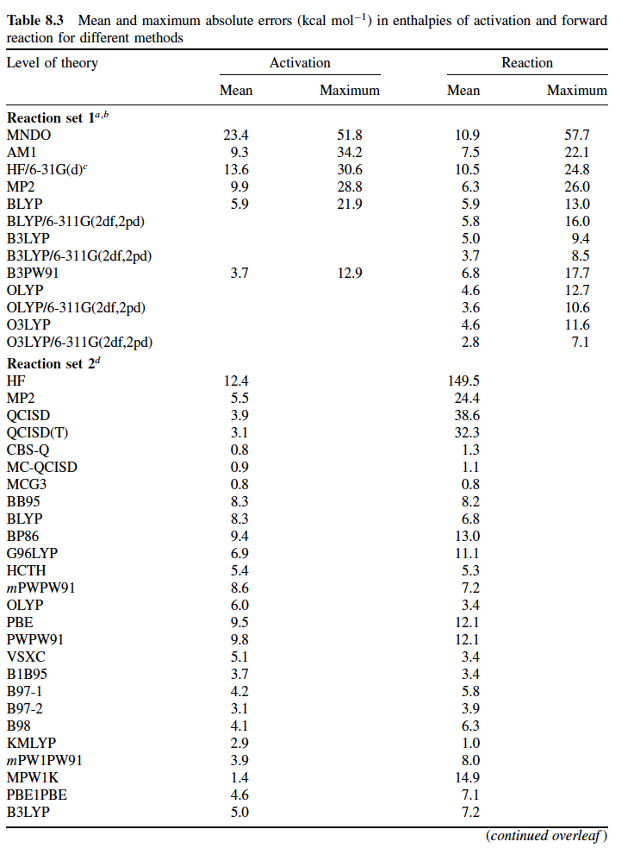
\includegraphics[width=0.8\linewidth]{lectures/figures/6_rxn_energies1.png}
    \end{figure}

\column{0.6\textwidth}
\begin{figure}
    \centering
    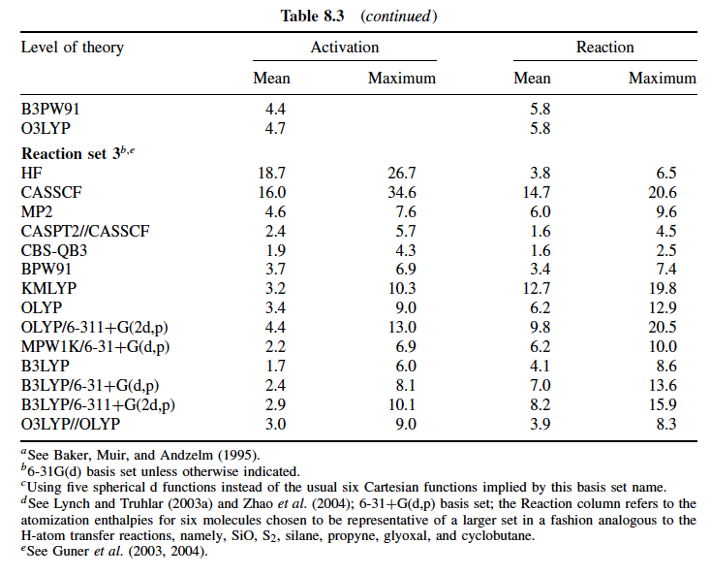
\includegraphics[width=0.5\linewidth]{lectures/figures/6_rxn_energies2.png}
\end{figure}
Broad conclusions
\begin{itemize}
    \item GGA better than LDA.
    \item Hybrids (esp B3LYP) most efficient (good accuracy comparable to highly correlated methods).
\end{itemize}

\end{columns} 

\end{frame} 

\begin{frame}{Some systemic errors can be addressed by fitting to experiments}
\begin{figure}
    \centering
    \begin{subfigure}{0.35\textwidth}
    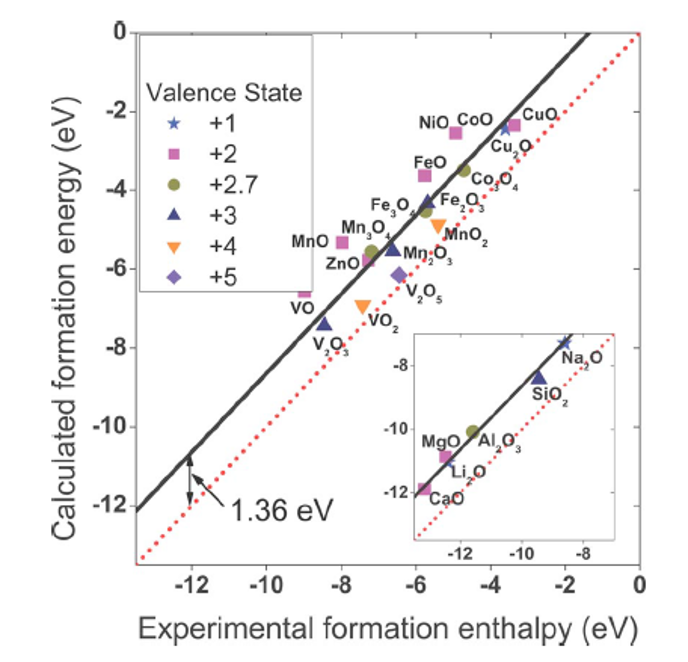
\includegraphics[width=\linewidth]{lectures/figures/6_oxidation_fitting.png}
    \caption{Ref \cite{wangOxidationEnergiesTransition2006}.}
    \end{subfigure}
    \begin{subfigure}{0.6\textwidth}
    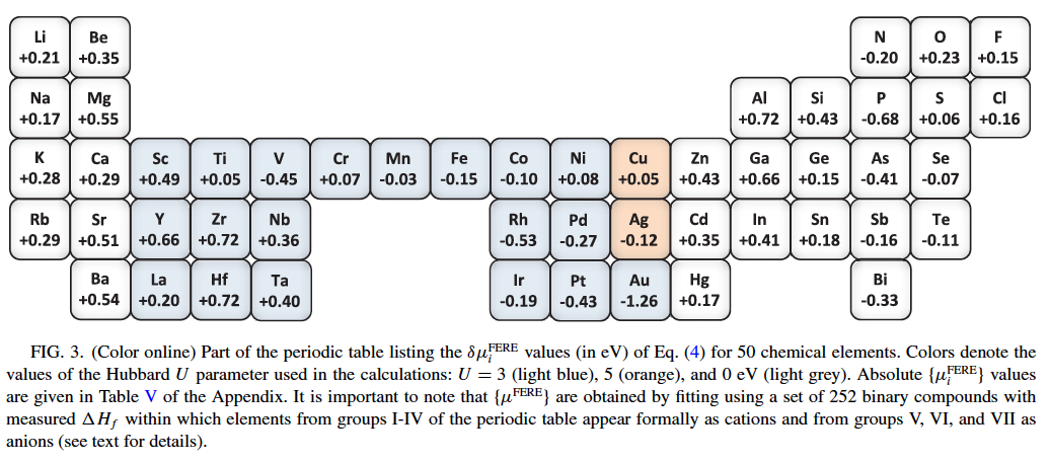
\includegraphics[width=\linewidth]{lectures/figures/6_oxidation_fitting2.png}
    \caption{Ref \cite{stevanovicCorrectingDensityFunctional2012}.}
    \end{subfigure}
    \end{figure}
\end{frame} 


\begin{frame}{If you know what you are doing, results can be pretty good...}
\begin{figure}
    \centering
    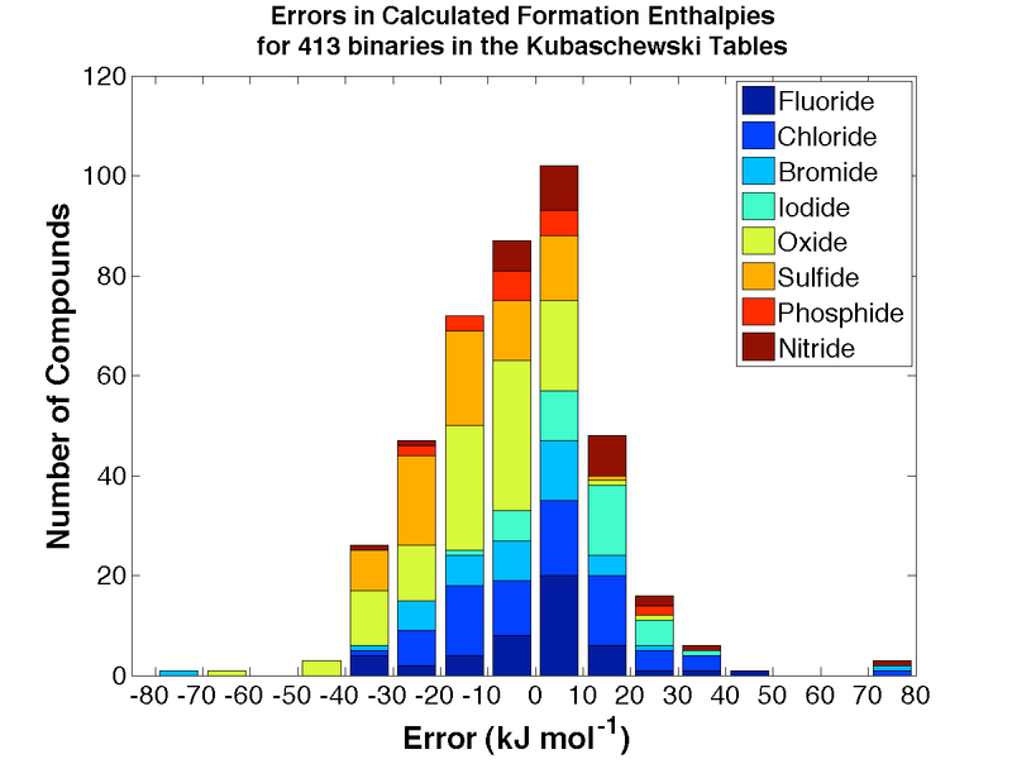
\includegraphics[width=0.5\linewidth]{lectures/figures/6_formation_energies_stats.png}
    \caption{High-throughput analysis using the Materials Project, again done by a UCSD NanoEngineering professor. See \href{https://docs.materialsproject.org/methodology/materials-methodology/thermodynamic-stability/thermodynamic-stability/anion-and-gga-gga+u-mixing}{MP docs}.}
    \end{figure}
\end{frame} 

\begin{frame}{Band gaps}
\begin{figure}
    \centering
    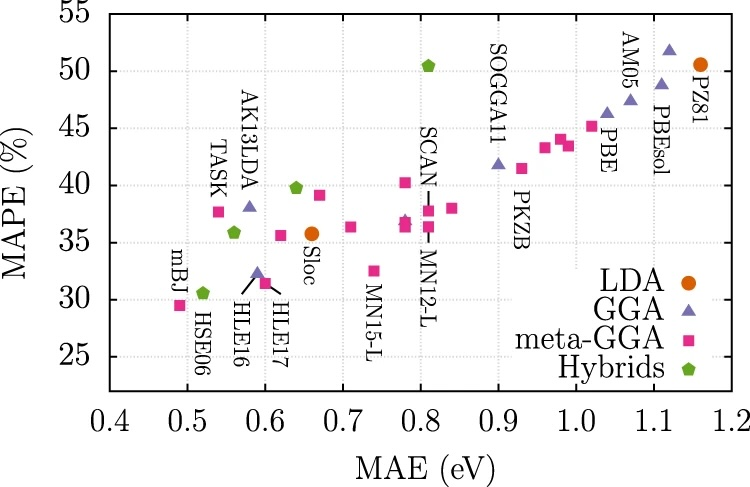
\includegraphics[width=0.55\linewidth]{lectures/figures/6_bandgaps.jpeg}
    \caption{Large-scale DFT theory study of 472 nonmagnetic materials, including covalent-, ionic-, and van der Waals-bonded solids.\cite{borlidoExchangecorrelationFunctionalsBand2020}}
    \end{figure}
\end{frame} 


\begin{frame}{Summary}
\begin{itemize}
    \item LDA underpredicts bond lengths, lattice parameters and overbinds.
    \item GGA error is smaller, but less systematic. But $< 1$\% in many cases.
    \item Band gaps are systematically underestimated in LDA and GGA. Meta-GGAs improve on this slightly. Hybrids can get much lower errors.
\end{itemize}

\begin{alertblock}{Conclusions}
\begin{itemize}
\item Very little reason to choose LDA over GGA since computational cost are similar.
\item Hybrids and state-of-the-art meta-GGAs such as SCAN provide significantly better results at increased computational cost.
\end{itemize}

\end{alertblock}

\end{frame} 


\begin{frame}[allowframebreaks]{Bibliography}
    \bibliographystyle{unsrt}
    \bibliography{refs}
\end{frame}



\begin{frame}
    \Huge{\centerline{The End}}
\end{frame}

\end{document}

